\subsection{Logistic-Normal via a Weighted Gaussian Process (\GPModel)}
\label{GP}

\begin{figure}
	\centering
	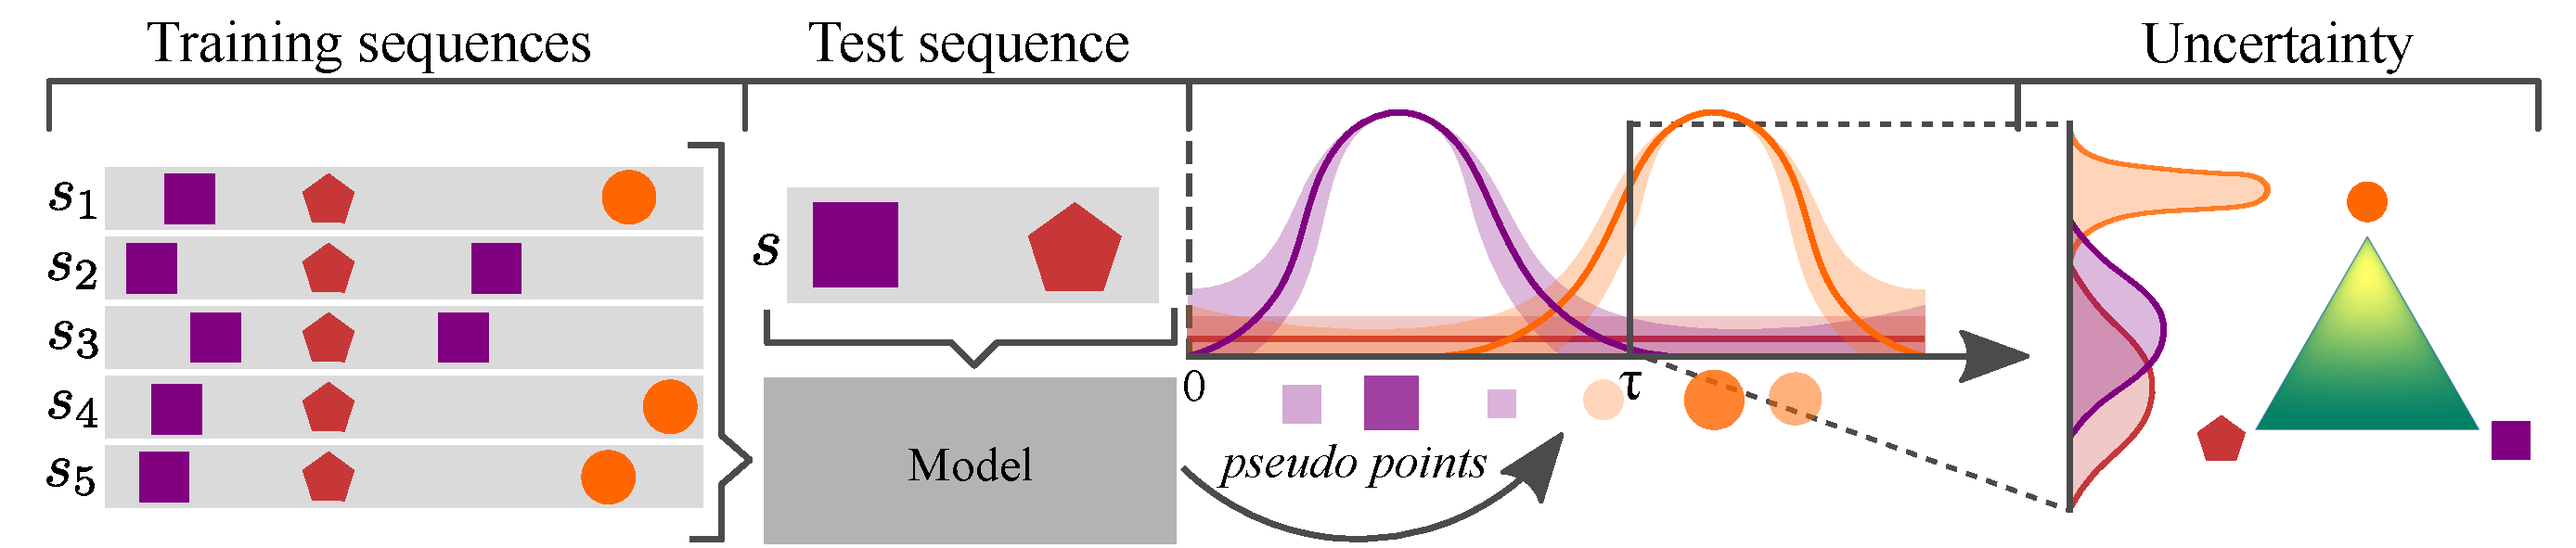
\includegraphics[width=\linewidth]{sections/010_neurips2019/paper/images/model_schema.pdf}
	\begin{subfigure}{0.3\textwidth}
		\caption{} \label{fig:model_illustration_1}
	\end{subfigure}
	\begin{subfigure}{0.69\textwidth}
		\caption{} \label{fig:model_illustration_2}
	\end{subfigure}
	\vspace*{-0.5cm}
    \caption{The model framework. (a) During training we use sequences $s_i$. (b) Given a new sequence of events $s$ the model generates pseudo points that describe $\bm{\theta}(\DeltaTime)$, i.e. the temporal evolution of the distribution on the simplex. These pseudo points are based on the data that was observed in the training examples and weighted accordingly. We also have a measure of certainty in our prediction.}\label{fig:model_illustration}
    \vspace*{-0.5cm}
\end{figure}

We start by describing our model for the case when $P$ is the family of logistic-normal (LN) distributions.
How to model a compact yet expressive evolution of the LN distribution?
Our core idea is to exploit the fact that the LN distribution corresponds to a multivariate random variable whose \textit{logits} follow a \textit{normal distribution} -- and a natural way to model the evolution of a normal distribution is a \textit{Gaussian Process}. Given this insight, the core idea of our model is illustrated in \cref{fig:model_illustration}: (1) we generate $\NbPoints$ pseudo points based on a hidden state of an RNN whose input is a sequence, (2) we fit a Gaussian Process to the pseudo points, thus capturing the temporal evolution, and (3) we use the learned GP for estimating the parameters $\bm \mu(\DeltaTime)$ and $\bm \Sigma(\DeltaTime)$ of the final LN distribution at any specific time $\tau$. Thus, by generating a small number of points we characterize the full distribution.

\paragraph{Classic GP.}  To keep the complexity low, we train one GP per class $\IndexClass$. That is, our model generates $\NbPoints$ points $(\DeltaTime_\IndexPoint^{(\IndexClass)}, y_\IndexPoint^{(\IndexClass)})$ per class $\IndexClass$, where $y_\IndexPoint^{(\IndexClass)}$ represents logits. Note that the first coordinate of each pseudo point corresponds to time, leading to the temporal evolution when fitting the GP. Essentially we perform a non-parameteric regression from the time domain to the logit space. Indeed, using a classic GP along with the pseudo points, the parameters $\theta$ of the logistic-normal distribution, $\bm \mu$ and $\bm \Sigma$, can be easily computed for any time $\tau$ in closed form:
\begin{equation}\label{eq:gp_prediction}
\begin{aligned}
\mu_{\IndexClass}(\DeltaTime) = \bm{k}_{\IndexClass}^T \bm{K}_{\IndexClass}^{-1} \bm{y}_{\IndexClass},\
\sigma_{\IndexClass}^2(\DeltaTime) = s_{\IndexClass} - \bm{k}_{\IndexClass}^T \bm{K}_{\IndexClass}^{-1} \bm{k}_{\IndexClass}
\end{aligned}
\end{equation}
where  $\bm K_c$ is the  gram matrix w.r.t.\ the $M$ pseudo points of class $c$ based on a  kernel $k$ (e.g. $\smash{k(\DeltaTime_1, \DeltaTime_2) = \exp( -\gamma^2 (\DeltaTime_1 - \DeltaTime_2)^2)}$). Vector $\bm{k}_{\IndexClass}$ contains at position $j$ the value $\smash{k(\DeltaTime_\IndexPoint^{(\IndexClass)},\tau)}$, and $\bm{y}_{\IndexClass}$ the value $\smash{y_\IndexPoint^{(\IndexClass)}}$, and $s_{\IndexClass}=k(\DeltaTime, \DeltaTime)$. At every time point $\DeltaTime$ the logits then follow a multivariate normal distribution with mean $\bm \mu(\DeltaTime)$ and covariance $\smash{\bm \Sigma = \text{diag}(\bm \sigma^2(\DeltaTime))}$.

Using a GP enables us to describe complex functions. Furthermore, since a GP models uncertainty in the prediction depending on the pseudo points, uncertainty is higher in areas far away from the pseudo points. Specifically, it holds for distant future; thus, matching the idea of locality.
%
However, uncertainty is always low around the $M$ pseudo points. Thus $\NbPoints$ should be carefully picked since there is a trade-off between having high certainty at (too) many time points and the ability to capture complex behavior. Thus, in the following we present an extended version solving this problem.

%\begin{wrapfigure}{r}{7cm}
\begin{figure}
	%\vspace*{-0.5cm}
    \centering
    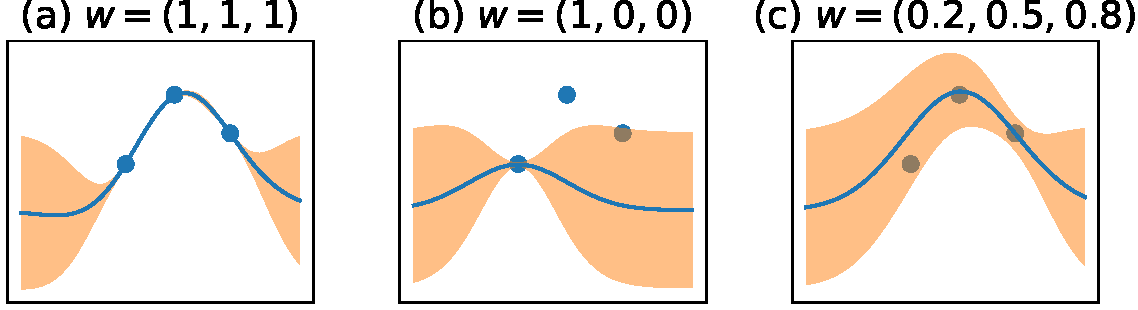
\includegraphics[width=0.8\linewidth]{sections/010_neurips2019/paper/images/weighted_gaussian_process.pdf}
	\caption{WGP on toy data with different weights. (a) All weights are 1 -- classic GP. (b) Zero weights discard points. (c) Mixed weight assignment.}
	\label{fig:weighted_gaussian_process}
%\vspace*{-0.5cm}
\end{figure}
%\end{wrapfigure}

%%%%% Horizontal %%%%%%
%\begin{figure}[H]
%\centering
%\scalebox{0.9}{\begin{tikzpicture}[
%rectanglenode/.style={rectangle, draw=black!100, very thick, minimum size=10mm},
%roundnode/.style={circle, draw=black!100, very thick, minimum size=10mm},
%nonenode/.style={rectangle, draw=none, minimum size=6mm},
%]
%\tikzset{edge/.style = {->,> = latex'}}
%\node[nonenode] (H)         at (-5.9, 10.25)       {$\History$};
%\node[nonenode] (e)      at (-5.9, 9.75)       {$e$};
%\node[rectanglenode] (RNN)       at (-4.5, 10)       {RNN};
%\node[nonenode] (pi)        at (-3, 9.5)       {$w_\IndexPoint^{(\IndexClass)}$};
%\node[nonenode] (mu)       at (-3, 10)       {$\DeltaTime_\IndexPoint^{(\IndexClass)}$};
%\node[nonenode] (sigma)        at (-3,10.5)       {$y_\IndexPoint^{(\IndexClass)}$};
%\node[nonenode] (alpha)        at (-1.5, 10)       {$\theta(\DeltaTime)$};
%\node[nonenode] (p)        at (0.75, 10)       {$\bm{p}(\DeltaTime) \sim P(\theta(\DeltaTime))$};
%\draw[edge] (H) -> (RNN) {};
%\draw[edge] (e) -> (RNN) {};
%\draw[edge] (RNN) -> (pi) {};
%\draw[edge] (RNN) -> (mu) {};
%\draw[edge] (RNN) -> (sigma) {};
%\draw[edge] (pi) -> (alpha) {};
%\draw[edge] (mu) -> (alpha) {};
%\draw[edge] (sigma) -> (alpha) {};
%\draw[edge] (alpha) -> (p) {};
%\end{tikzpicture}}
%\caption{Model diagram. Both models output pseudo points given history and new event. In \GPModel they generate parameters $\theta(\DeltaTime) = \{\bm \mu (\DeltaTime), \bm \Sigma(\DeltaTime)\}$ that model $P(\theta(\DeltaTime))$ as a logistic-normal distribution. In \DirModel these points generate $\theta(\DeltaTime) = \bm \alpha(\DeltaTime)$ to model $P(\theta(\DeltaTime))$ as a Dirichlet distribution.}
%\label{fig:model_diagram}
%\end{figure}
%%%%% Vertical %%%%%%
% \InsertBoxR{3}{\parbox{0.3\linewidth}{
\begin{wrapfigure}[12]{r}{3.5cm}
    \vspace*{-0.6cm}
    \centering
    \scalebox{.75}{\begin{tikzpicture}[
    rectanglenode/.style={rectangle, draw=black!100, very thick, minimum size=10mm},
    roundnode/.style={circle, draw=black!100, very thick, minimum size=5mm},
    nonenode/.style={rectangle, draw=none, minimum size=6mm},
    ]
    \tikzset{edge/.style = {->,> = latex'}}
    \node[nonenode] (H)         at (8.7,4.5)       {$\History_{\IndexEvent-1}$};
    \node[nonenode] (e)      at (10,5.6)       {$e_{\IndexEvent-1}$};
    \node[rectanglenode] (RNN)       at (10,4.5)       {RNN};
    \node[nonenode] (pi)        at (9.25,3.4)       {$[w_\IndexPoint^{(\IndexClass)},$};
    \node[nonenode] (mu)       at (10,3.4)       {$\DeltaTime_\IndexPoint^{(\IndexClass)},$};
    \node[nonenode] (sigma)        at (11,3.4)       {$y_\IndexPoint^{(\IndexClass)}]_{\IndexPoint=1}^\NbPoints$};
    \node[roundnode] (regression)        at (10,2.4)       {GP};
    \node[nonenode] (alpha)        at (10,1.4)       {$\DeltaTime_{\IndexClass}(\DeltaTime), \sigma_{\IndexClass}^2(\DeltaTime)$};
    \node[nonenode] (p)        at (10,0.5)       {$\bm{p}(\DeltaTime) \sim P(\theta(\DeltaTime))$};
    \draw[edge] (H) -> (RNN) {};
    \draw[edge] (e) -> (RNN) {};
    \draw[edge] (RNN) -> (pi) {};
    \draw[edge] (RNN) -> (mu) {};
    \draw[edge] (RNN) -> (sigma) {};
    \draw[edge] (pi) -> (regression) {};
    \draw[edge] (mu) -> (regression) {};
    \draw[edge] (sigma) -> (regression) {};
    \draw[edge] (regression) -> (alpha) {};
    \draw[edge] (alpha) -> (p) {};
    \end{tikzpicture}}
    \caption{Model diagram}\label{fig:model_diagram}
% }}[6]
    \vspace*{-1cm}
\end{wrapfigure}

\paragraph{Weighted GP.} We would like to pick $\NbPoints$ large enough to express rich multimodal functions and allow the model to discard unnecessary points.
To do this we generate an additional weight vector $\smash{\bm{w}^{(\IndexClass)} \in [0,1]^\NbPoints}$ that assigns the weight $\smash{w_\IndexPoint^{(\IndexClass)}}$ to a point $\smash{\DeltaTime^{(\IndexClass)}_\IndexPoint}$. Giving a zero weight to a point should discard it, and giving $1$ will return the same result as with a classic GP. To achieve this goal, we introduce a new kernel function:
\begin{equation}
\begin{aligned}\label{eq:weighted_kernel}
    k'(\DeltaTime_1, \DeltaTime_2) &= f(w_1, w_2) k(\DeltaTime_1, \DeltaTime_2)
\end{aligned}
\end{equation}
%\parskip 0pt
where $k$ is the same as above. The function $f$ weights the kernel $k$ according to the weigths for $\DeltaTime_1$ and $\DeltaTime_2$.
We require $f$ to have the following properties: (1) $f$ should be a valid kernel over the weights, since then the function $k'$ is a valid kernel as well; (2) the importance of pseudo points should not increase, giving $f(w_1, w_2) \leq \min(w_1,w_2)$; this fact implies that a point with zero weight will be discarded since $f(w_1, 0)=0$ as desired. The function $f(w_1,w_2)=\min(w_1,w_2)$  is a simple choice that fulfills these properties.
In \cref{fig:weighted_gaussian_process}  we show the effect of different weights when fitting of a GP (see app.~\ref{gp_min_kernel} for a more detailed discussion of the behavior of the $\min$ kernel).
%\parskip 5pt
To predict $\mu$ and $\sigma^2$ for a new time $\DeltaTime$, we can now simply apply \cref{eq:gp_prediction} based on the new kernel $k'$, where the weight for the \textit{query} point $\DeltaTime$ is $1$.

To summarize: From a hidden state $\smash{h_\IndexEvent = \text{RNN}(\Event_{\IndexEvent-1}, \History_{\IndexEvent-1})}$ we use a a neural network to generate $\NbPoints$ weighted pseudo points $(w_\IndexPoint^{(\IndexClass)}, \DeltaTime_\IndexPoint^{(\IndexClass)}, x_\IndexPoint^{(\IndexClass)})$ per class $\IndexClass$.
Fitting a Weighted GP to these points enables us to model the temporal evolution of $\smash{\mathcal{N}(\mu_\IndexClass(\DeltaTime), \sigma_\IndexClass^2(\DeltaTime))}$ and, thus, accordingly of the logistic-Normal distribution. \cref{fig:model_diagram} shows an illustration of this model.
%
Note that the cubic complexity of a GP, due to the matrix inversion, is not an issue since the number $\NbPoints$ is usually small ($<10$), while still allowing to represent rich multimodal functions. Crucially, given the loss defined in \cref{uncertainty_loss}, our model is fully differentiable, enabling us efficient training.